\pdfminorversion=4
\documentclass[aspectratio=169]{beamer}

\mode<presentation>
{
  \usetheme{default}
  \usecolortheme{default}
  \usefonttheme{default}
  \setbeamertemplate{navigation symbols}{}
  \setbeamertemplate{caption}[numbered]
  \setbeamertemplate{footline}[frame number]  % or "page number"
  \setbeamercolor{frametitle}{fg=white}
  \setbeamercolor{footline}{fg=black}
} 

\usepackage[english]{babel}
\usepackage{inputenc}
\usepackage{tikz}
\usepackage{courier}
\usepackage{array}
\usepackage{bold-extra}
\usepackage{minted}
\usepackage[thicklines]{cancel}
\usepackage{fancyvrb}

\xdefinecolor{dianablue}{rgb}{0.18,0.24,0.31}
\xdefinecolor{darkblue}{rgb}{0.1,0.1,0.7}
\xdefinecolor{darkgreen}{rgb}{0,0.5,0}
\xdefinecolor{darkgrey}{rgb}{0.35,0.35,0.35}
\xdefinecolor{darkorange}{rgb}{0.8,0.5,0}
\xdefinecolor{darkred}{rgb}{0.7,0,0}
\definecolor{darkgreen}{rgb}{0,0.6,0}
\definecolor{mauve}{rgb}{0.58,0,0.82}

\title[2024-12-17-complex-step-autodiff]{Awkward Array's JAX backend and \\ complex-step autodiff as an alternative}
\author{Jim Pivarski}
\institute{Princeton University -- IRIS-HEP}
\date{December 17, 2024}

\usetikzlibrary{shapes.callouts}

\begin{document}

\logo{\pgfputat{\pgfxy(0.11, 7.4)}{\pgfbox[right,base]{\tikz{\filldraw[fill=dianablue, draw=none] (0 cm, 0 cm) rectangle (50 cm, 1 cm);}\mbox{\hspace{-8 cm}
\includegraphics[height=1 cm]{princeton-logo-long.png}\hspace{0.1 cm}\raisebox{0.1 cm}{
\includegraphics[height=0.8 cm]{iris-hep-logo-long.png}}\hspace{0.1 cm}}}}}

\begin{frame}
  \titlepage
\end{frame}

\logo{\pgfputat{\pgfxy(0.11, 7.4)}{\pgfbox[right,base]{\tikz{\filldraw[fill=dianablue, draw=none] (0 cm, 0 cm) rectangle (50 cm, 1 cm);}\mbox{\hspace{-8 cm}
\includegraphics[height=1 cm]{princeton-logo.png}\hspace{0.1 cm}\raisebox{0.1 cm}{
\includegraphics[height=0.8 cm]{iris-hep-logo.png}}\hspace{0.1 cm}}}}}

% Uncomment these lines for an automatically generated outline.
%\begin{frame}{Outline}
%  \tableofcontents
%\end{frame}

% START START START START START START START START START START START START START

\begin{frame}{Awkward Array has 4 backends}
\large
\vspace{0.5 cm}
\begin{itemize}\setlength{\itemsep}{0.5 cm}
\item<1-> \mintinline{python}{"cpu"}: buffers (user data, indexes, offsets, etc.) are NumPy arrays, computations are performed by NumPy functions or cpu-kernels.so
\item<2-> \mintinline{python}{"cuda"}: buffers are CuPy arrays, CUDA kernels are JIT-compiled by CuPy
\item<3-> \mintinline{python}{"typetracer"}: buffers are dataless Python objects that only infer types (intended for Dask; currently only used by Dask)
\item<4-> \mintinline{python}{"jax"}: data buffers are JAX arrays, indexes are NumPy, \mintinline{python}{ak.Array} is flattened/unflattened as PyTrees
\end{itemize}

\vspace{0.5 cm}
\uncover<5->{When a backend is untested, it gets out of date. \mintinline{python}{"jax"} has 44 tests. (\mintinline{python}{"cuda"} has 459 tests and \mintinline{python}{"cpu"} + \mintinline{python}{"typetracer"} has 2214 tests and are used daily.)}
\end{frame}

\begin{frame}{JAX backend development}
\large
\vspace{0.5 cm}
\begin{columns}
\column{1.1\linewidth}
\only<1>{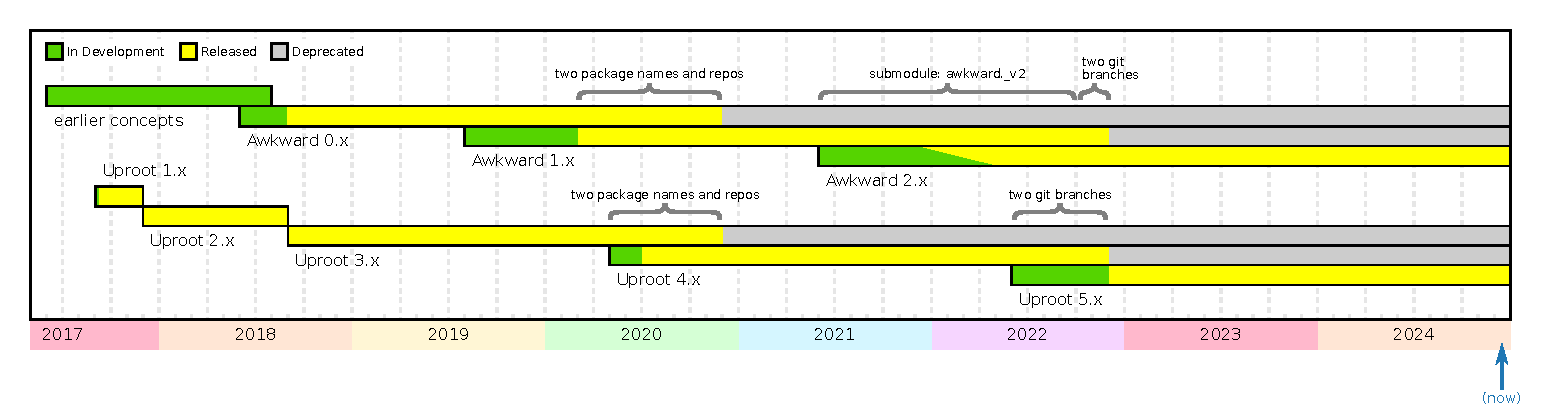
\includegraphics[width=\linewidth]{awkward-uproot-timeline.pdf}}\only<2->{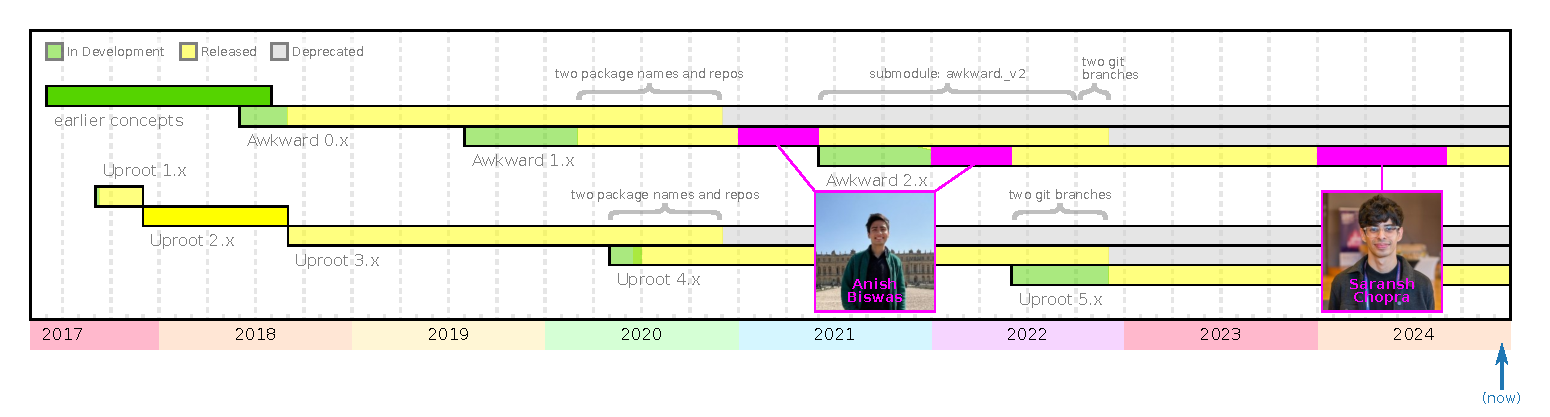
\includegraphics[width=\linewidth]{awkward-uproot-timeline-jax.pdf}}
\end{columns}

\begin{uncoverenv}<2->
\begin{itemize}\setlength{\itemsep}{0.25 cm}
\item<2-> Jan 2021--Apr 2021: Anish Biswas as IRIS-HEP Fellow
\begin{itemize}
\item wasn't possible at all, motivated Awkward v2 C++ $\to$ Python reimplementation
\end{itemize}
\item<3-> Jan 2022--Jun 2022: Anish Biswas as CERN Contractor
\begin{itemize}
\item implemented map-like functions in PyTrees, reduce-like functions with LAX
\end{itemize}
\item<4-> Jan 2024--Sep 2024: Saransh Chopra as IRIS-HEP Gap Year Fellow
\begin{itemize}
\item ``on call'' for feedback from autograd users; received very little
\end{itemize}
\end{itemize}
\end{uncoverenv}
\end{frame}

\begin{frame}{Limitations on the JAX backend}
\large
\vspace{0.5 cm}
\begin{itemize}\setlength{\itemsep}{0.5 cm}
\item<1-> JAX's JIT-compilation is a non-starter: XLA requires array sizes to not be dependent on data values at compile-time, and that rule is broken throughout Awkward's codebase.
\item<2-> JAX's PyTree extension mechanism exclusively works on map-like operations: $f(\vec{x}) = f(x_i)$ for all components $x_i$ of array $\vec{x}$.
\item<3-> We were lucky enough that JAX's LAX library has segmented reductions.
\item<4-> I'm not completely sure all of the above works: Anish was fighting corner cases to the end and we don't have much user feedback.
\end{itemize}
\end{frame}

\begin{frame}{Occasionally, the JAX tests fail and are patched}
\vspace{0.25 cm}
\begin{columns}
\column{0.55\linewidth}
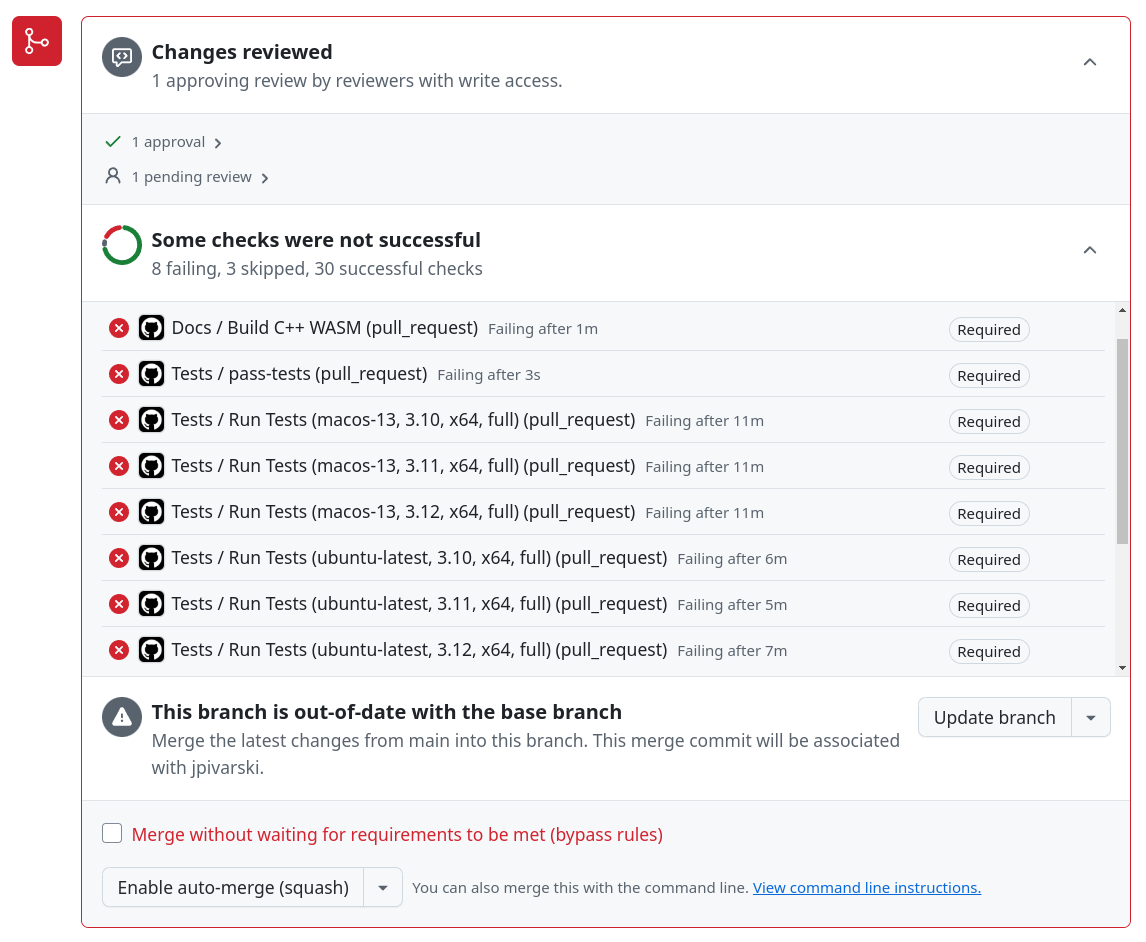
\includegraphics[width=\linewidth]{jax-failures.png}

\column{0.5\linewidth}
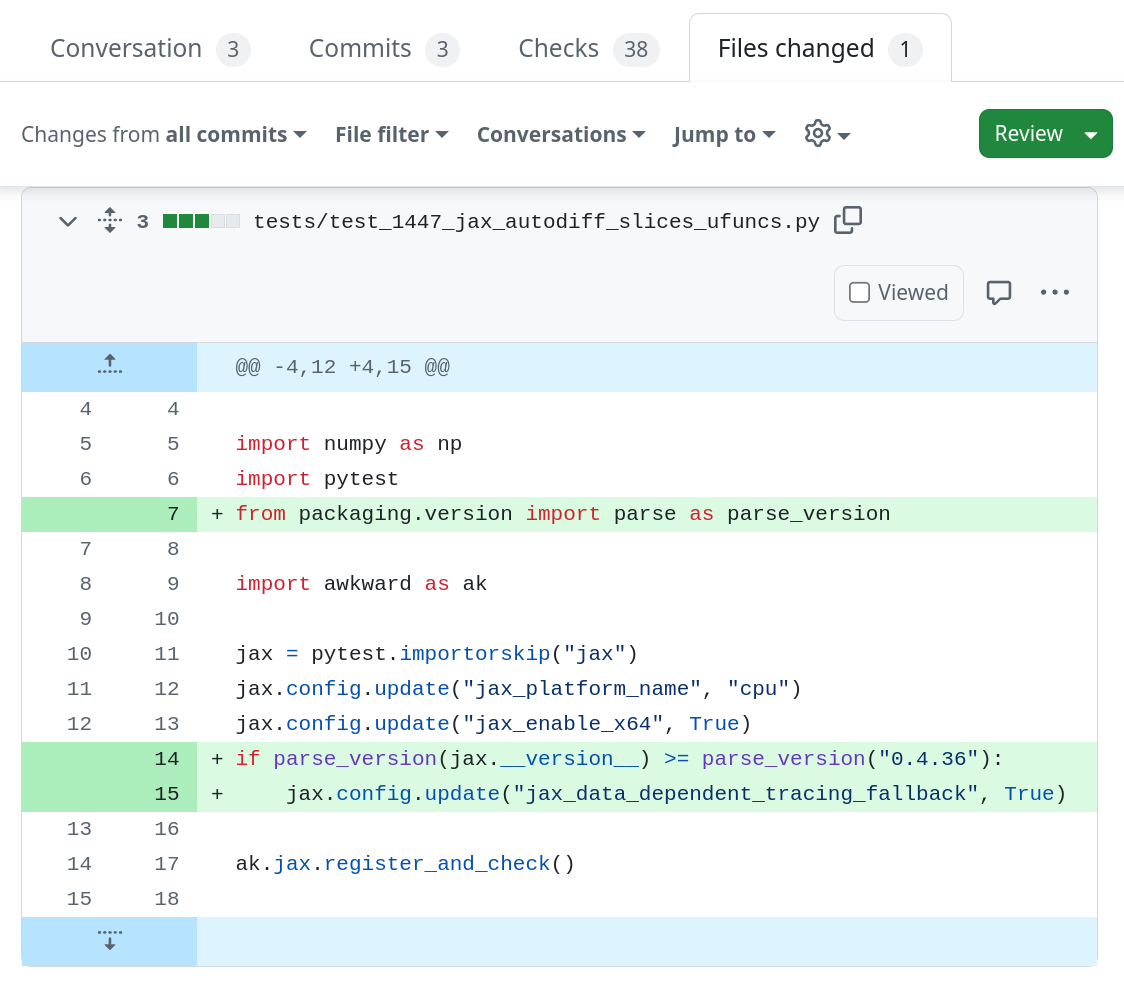
\includegraphics[width=\linewidth]{jax-failures-2.png}
\end{columns}
\end{frame}

\begin{frame}{Can we get autodiff without JAX?}
\large
\vspace{0.5 cm}
\begin{itemize}\setlength{\itemsep}{0.5 cm}
\item<1-> HIPS/autograd is a simpler library; Awkward v1's PR \#120 wraps \mintinline{python}{elementwise_grad} (forward autodiff of mappers as a dectorator).
\item<2-> If forward autodiff is acceptable, a backend based on an eager primal + tangent array would let us control program flow and get 100\% coverage.
\item<3-> If backpropagation is necessary, we could at least get dask-awkward's coverage by using our own typetracer or Dask DAGs.
\item<4-> How hard is it to implement autodiff, anyway?
\end{itemize}
\end{frame}

%% \begin{frame}{Theory of autodiff: complex numbers}
%% \vspace{0.25 cm}
%% {\scriptsize \textcolor{blue}{\url{https://www.hedonisticlearning.com/posts/complex-step-differentiation.html}}}

%% \vspace{0.3 cm}
%% Given an infinitely differentiable function $f : \Bbb{R} \to \Bbb{R}$, consider a complex extension $F : \Bbb{C} \to \Bbb{C}$ with $F(x) = f(x)$ for $x \in \Bbb{R}$. ($F$ is ``holomorphic'' or ``complex analytic.'')

%% \vspace{0.3 cm}
%% \begin{uncoverenv}<2->
%% Using midpoint rule integration in a circle of radius $h > 0$ around $x$ at 2 points:

%% \[ F'(x) \approx \frac{1}{2hi} \bigg[F(x + hi) - F(x - hi) \bigg] \]
%% \end{uncoverenv}

%% \begin{uncoverenv}<3->
%% Since $F(\overline{z}) = \overline{F(z)}$, the expression in brackets is $2i\,\mbox{Im}\big(f(x + hi)\big)$ and

%% \[ F'(x) \approx \mbox{Im} \bigg( F(x + hi) \bigg) / h \]
%% \end{uncoverenv}

%% \uncover<4->{(Unlike the finite difference method, there's no subtraction of real values.)}
%% \end{frame}

%% \begin{frame}{Theory of autodiff: what JAX and other libraries do}
%% The equation for complex-valued $F$

%% \[ F'(x) \approx \mbox{Im} \bigg( F(x + hi) \bigg) / h \]

%% becomes exact if $h > 0$ and $h^2 = 0$. There's an algebraic ring with this property called ``dual numbers,'' which 

%% \end{frame}

\begin{frame}{Theory of autodiff: complex numbers}
\vspace{0.3 cm}
{\scriptsize \textcolor{blue}{\url{https://www.hedonisticlearning.com/posts/complex-step-differentiation.html}}}

{\scriptsize \textcolor{blue}{\url{https://researchrepository.wvu.edu/faculty_publications/426}}}

\vspace{0.3 cm}
Calculating a derivative of $f : \Bbb{R} \to \Bbb{R}$ to $\mathcal{O}(h^2)$ by finite differences:

\[ f'(x) \approx \frac{1}{2h} \bigg( f(x + h) - f(x - h) \bigg) \]

but too-small $h$ has large cancellations and too-large $h$ steps over bumps in $f$.

\vspace{0.3 cm}
\begin{uncoverenv}<2->
Instead, take a step $h = i\varepsilon$ on a function $F(z) = f(z)$ for $z \in \Bbb{R}$ with $F(\overline{z}) = \overline{F(z)}$:

\[ F'(x) \approx \frac{1}{2\varepsilon} \bigg( F(x + i\varepsilon) - F(x - i\varepsilon) \bigg) = \frac{1}{\varepsilon} \mbox{Im}\bigg( F(x + i\varepsilon) \bigg) \]
\end{uncoverenv}

\vspace{0.3 cm}
\uncover<3->{No more additive cancellations and the step is perpendicular to bumps in $f$.}
\end{frame}

\begin{frame}{Theory of autodiff: dual numbers}
\vspace{0.3 cm}
The derivative of $f$ from its complex extension $F$,

\[ f'(x) \approx \mbox{Im}\bigg( F(x + i\varepsilon) \bigg) / \varepsilon \]

is exact if $\varepsilon > 0$ and $\varepsilon^2 = 0$. The complex numbers don't have this property, but imagine an abstract algebra in which this is true.

\vspace{0.3 cm}
\uncover<2->{This algebra is called ``dual numbers,'' and it's the space-time extension used in SUSY. The Taylor expansion of a quantum field in superspace has exactly 2 terms, identified as a fermion field and a boson field.}

\vspace{0.3 cm}
\uncover<3->{For autodiff, the two components are the primal array and tangent array. Implementing autodiff is as hard as implementing complex extensions for every real function.}

\vspace{0.3 cm}
\uncover<4->{But if we already have a complex implementation of all of our functions, we can set $\varepsilon = 10^{-8}$ to get $10^{-16}$ errors (typical errors in double-precision floating-point).}
\end{frame}

\begin{frame}[fragile]{A complete autodiff library on one slide (NumPy \& CuPy)}
\vspace{0.1 cm}
\tiny
\begin{columns}
\column{0.55\linewidth}
\begin{minted}{python}
import numpy as np
from numpy.lib.mixins import NDArrayOperatorsMixin

class diffarray(NDArrayOperatorsMixin):
    @classmethod
    def _build(cls, complex_array):
        self = cls.__new__(cls); self._array = complex_array
        return self

    def __init__(self, primal, tangent=None):
        if issubclass(primal.dtype.type, np.float32):
            self._array = primal.astype(np.complex64)
        elif issubclass(primal.dtype.type, np.float64):
            self._array = primal.astype(np.complex128)
        else:
            raise TypeError("array must be float32 or float64")
        if tangent is None:
            self._array += 1j * self._step_scale
        else:
            self._array += tangent * 1j * self._step_scale
    @property
    def _step_scale(self):
        return 1e-4 if issubclass(
            self._array.dtype.type, np.complex128) else 1e-8

    @property
    def primal(self):
        return np.real(self._array)
    @property
    def tangent(self):
        return np.imag(self._array) / self._step_scale
\end{minted}

\column{0.55\linewidth}
\begin{minted}{python}
def __array_ufunc__(self, ufunc, method, *args, **kwargs):
    return self.__array_function__(ufunc, None, args, kwargs)

def __array_function__(self, func, types, args, kwargs):
    # functions that would be misinterpreted on complex
    if func.__name__ == "abs":
        out = args[0].copy()
        out[out.real < 0] *= -1
        return type(self)._build(out)
    if func.__name__ == "real":
        return type(self)._build(args[0]._array)
    if func.__name__ == "imag":
        return type(self)._build(args[0]._array * 0)
    if func.__name__ in ("less", "less_equal", "equal",
                   "not_equal", "greater", "greater_equal"):
        args = [getattr(x, "_array", x).real for x in args]
        return func(*args, **kwargs)

    # all other functions
    args = [getattr(x, "_array", x) for x in args]
    kwargs = {
        k: getattr(v, "_array", v) for k, v in kwargs.items()
    }
    out = func(*args, **kwargs)
    return type(self)._build(out) if issubclass(
        out.dtype.type, np.complexfloating) else out

def __getitem__(self, where):
    out = self._array[where]
    return type(self)._build(np.asarray(out)) if isinstance(
        out, np.complexfloating) else out
\end{minted}
\end{columns}
\end{frame}

\begin{frame}[fragile]{A complete autodiff library on one slide (NumPy \& CuPy)}
\vspace{0.2 cm}
\scriptsize
\begin{minted}{python}
>>> import numpy as np
>>> import matplotlib.pyplot as plt

>>> x = np.linspace(-20, 20, 10000)
>>> da_x = diffarray(x)
>>> da_y = np.sin(da_x) / da_x
>>> abs(da_y.tangent - ((x*np.cos(x) - np.sin(x)) / x**2)).max()
3.9683650809863025e-10

>>> plt.plot(x, da_y.tangent)
>>> plt.plot(x, (x*np.cos(x) - np.sin(x)) / x**2, ls="--")
\end{minted}

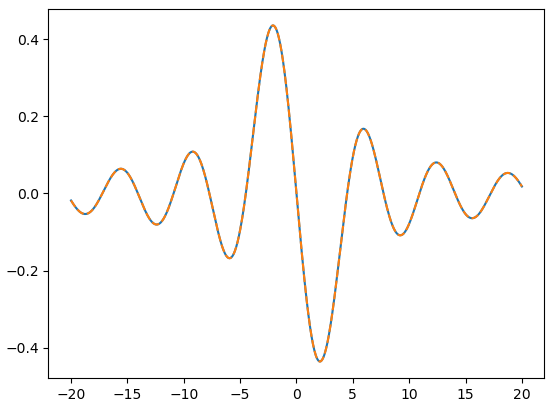
\includegraphics[width=0.4\linewidth]{autodiff-plot.png}
\end{frame}

\begin{frame}{So, what's wrong with it?}
\large
\vspace{0.5 cm}
\begin{itemize}\setlength{\itemsep}{0.5 cm}
\item<1-> Bad stuff happens at points where the function isn't infinitely differentiable (same for other autodiff libraries: consider the derivative of ReLU).
\item<2-> Can we do second (or higher) order derivatives? No. {\scriptsize(\textcolor{blue}{\url{https://dl.acm.org/doi/10.1145/2168773.2168774}})}
\item<3-> Differentiate with respect to multiple arguments? Probably!
\item<4-> Backpropagation: we might need to use our typetracer and/or Dask DAGs.
\item<5-> Usable in Numba: in principle, and that's an interesting possibility, considering that JAX can't and applying e.g.\ Enzyme is complicated.
\end{itemize}

\vspace{0.5 cm}
\uncover<6->{What else? Can anyone find a reason why this is not sufficient?}
\end{frame}

\begin{frame}{What are our options?}
\large
\vspace{0.5 cm}
\begin{enumerate}\setlength{\itemsep}{0.5 cm}
\item Keep the JAX backend in Awkward Array, tweaking as necessary.
\item Drop the JAX backend and\ldots\vspace{0.25 cm}
\begin{enumerate}\setlength{\itemsep}{0.25 cm}\large
\item give up on autodiff.
\item make a new autodiff mini-library that is Awkward-friendly that\ldots\vspace{0.125 cm}
\begin{enumerate}\setlength{\itemsep}{0.125 cm}\large
\item just uses the complex-valued implementations we already have.
\item implements a conventional autodiff.
\end{enumerate}
\item hide an autodiff implementation inside Awkward that\ldots\vspace{0.125 cm}
\begin{enumerate}\setlength{\itemsep}{0.125 cm}\large
\item just uses the complex-valued implementations we already have.
\item implements a conventional autodiff.
\end{enumerate}
\end{enumerate}
\end{enumerate}
\end{frame}

\end{document}
